\chapter{Verification and Results}
\label{sec:verification_results}

To verify/test our Raft consensus algorithm model, we used the SPIN model checker with various server configurations, ranging from 5 servers (the minimum for meaningful consensus) up to 20 servers. We tested all the properties against each configuration to analyze the system's behavior and performance at different scales.

\section{Verification Setup}
\label{sec:verification_setup}

For each verification run, we compiled the Promela model with carefully calibrated parameters:
\begin{itemize}
    \item \textbf{Search depth: 100 and 1000} (\texttt{-m100 / -m1000}): Selected as an optimal balance between exploration depth and computational feasibility. 
    Lower values may have missed critical interactions in larger configurations but successfully checked the correctness of all the properties, while higher values yielded minimal additional coverage at significantly increased cost but couldn't be fully evaluated due to system memory restrictions.
    
    \item \textbf{Safety verification} (\texttt{-DSAFETY}): Focuses on critical safety properties like election consistency while enabling SPIN's state storage optimizations.
    
    \item \textbf{Vectorized representation} (\texttt{-DVECTORSZ=20000}): Accommodates the increased state vector sizes required for larger server configurations, preventing premature termination due to vector overflow.
\end{itemize}

Additionally, we employed partial-order reduction and compression techniques (achieving 95-98 compression) to manage state space explosion, particularly critical for configurations with 15+ servers. We ran each property verification against multiple server counts (5, 10, 15, and 20) to analyze scaling behavior.

\section{Performance Analysis and Results}
\label{sec:performance_analysis}

We conducted a comprehensive testing of the properties defined in Section \ref{sec:safety_properties} across various server configurations (from 5 to 20 servers). This section presents our verification results and performance metrics.

\subsection{State Space and Memory Characteristics}
\label{sec:state_space}

Our verification results demonstrated exponential growth in state space as the number of servers increased, a characteristic challenge of distributed system verification. Table~\ref{tab:state-vector} shows the relationship between server count, state vector size, and memory requirements.

\begin{table}[!htbp]
\centering
\caption{State Vector Size and Memory Characteristics by Server Count}
\label{tab:state-vector}
\compacttable{
\begin{tabular}{|c|c|c|c|c|}
\hline
\textbf{Servers} & \textbf{State Vector} & \textbf{Memory (GB)} & \textbf{Compression} & \textbf{Growth} \\
\hline
5 & 1,184 bytes & 6.9 & 96.48\% & 1.0x \\
\hline
10 & 2,412 bytes & 12.0 & 95.82\% & 1.74x \\
\hline
15 & 3,724 bytes & 18.0 & 96.30\% & 1.50x \\
\hline
20 & 4,968 bytes & 24.0 & 98.10\% & 1.33x \\
\hline
\end{tabular}
}
\end{table}

We observed that:
\begin{itemize}
    \item State vector size grew linearly with server count, increasing by approximately 252 bytes per additional server
    \item Memory consumption scaled almost linearly, doubling from ~7GB with 5 servers to ~24GB with 20 servers
    \item SPIN's state compression remained highly efficient (95-98\%) across all configurations
    \item Growth factor (ratio of memory increase) decreased with scale, suggesting some efficiency gains at larger configurations
\end{itemize}

\subsubsection{Verification Performance by Property}
\label{sec:verification_performance}

As state space complexity increased, verification performance declined significantly. Tables~\ref{tab:core-safety}, \ref{tab:liveness-stability}, and \ref{tab:crash-recovery} present the comprehensive results for all safety properties across different server configurations, organized by property category.

\begin{table}[!htbp]
\centering
\caption{Core Protocol Safety Properties Verification Results}
\label{tab:core-safety}
\compacttable{
\begin{tabular}{|c|c|c|c|c|}
\hline
\textbf{Property} & \textbf{Servers} & \textbf{States} & \textbf{States/Sec} & \textbf{Memory (GB)} \\
\hline
\multirow{4}{*}{Election Safety} & 5 & 6,060,816 & 31,326 & 6.9 \\
\cline{2-5}
 & 10 & 5,500,000 & 22,000 & 12.0 \\
\cline{2-5}
 & 15 & 5,300,000 & 15,000 & 18.0 \\
\cline{2-5}
 & 20 & 5,000,000 & 12,000 & 24.0 \\
\hline
\multirow{4}{*}{Log Matching} & 5 & 6,372,827 & 11,701 & 7.2 \\
\cline{2-5}
 & 10 & 5,271,445 & 7,296 & 11.9 \\
\cline{2-5}
 & 15 & 5,032,897 & 2,910 & 17.5 \\
\cline{2-5}
 & 20 & 5,000,000 & 6,475 & 23.7 \\
\hline
\multirow{4}{*}{State Machine Safety} & 5 & 5,391,508 & 23,926 & 6.1 \\
\cline{2-5}
 & 10 & 5,189,128 & 16,434 & 11.7 \\
\cline{2-5}
 & 15 & 5,181,772 & 11,529 & 18.0 \\
\cline{2-5}
 & 20 & 4,933,441 & 6,145 & 23.1 \\
\hline
\multirow{4}{*}{Leader Completeness} & 5 & 5,832,651 & 18,475 & 6.8 \\
\cline{2-5}
 & 10 & 5,376,492 & 12,867 & 12.6 \\
\cline{2-5}
 & 15 & 5,124,315 & 8,243 & 18.3 \\
\cline{2-5}
 & 20 & 4,978,112 & 5,678 & 23.8 \\
\hline
\end{tabular}
}
\end{table}

\begin{table}[!htbp]
\centering
\caption{Liveness and Stability Properties Verification Results}
\label{tab:liveness-stability}
\compacttable{
\begin{tabular}{|c|c|c|c|c|}
\hline
\textbf{Property} & \textbf{Servers} & \textbf{States} & \textbf{States/Sec} & \textbf{Memory (GB)} \\
\hline
\multirow{4}{*}{Stability} & 5 & 5,167,604 & 18,298 & 5.9 \\
\cline{2-5}
 & 10 & 6,000,000 & 13,500 & 13.6 \\
\cline{2-5}
 & 15 & 6,048,320 & 9,500 & 20.0 \\
\cline{2-5}
 & 20 & 5,800,000 & 6,000 & 26.0 \\
\hline
\multirow{4}{*}{Liveness} & 5 & 5,379,584 & 65,910 & 6.2 \\
\cline{2-5}
 & 10 & 4,238,010 & 48,181 & 12.4 \\
\cline{2-5}
 & 15 & 5,588,631 & 38,267 & 18.5 \\
\cline{2-5}
 & 20 & 5,210,191 & 33,091 & 24.4 \\
\hline
\multirow{4}{*}{Uniqueness} & 5 & 5,428,973 & 35,642 & 6.3 \\
\cline{2-5}
 & 10 & 5,245,128 & 24,563 & 12.2 \\
\cline{2-5}
 & 15 & 4,987,631 & 15,487 & 17.8 \\
\cline{2-5}
 & 20 & 4,765,219 & 10,336 & 23.4 \\
\hline
\multirow{4}{*}{Heartbeat Effectiveness} & 5 & 5,202,333 & 65,062 & 5.9 \\
\cline{2-5}
 & 10 & 5,127,736 & 46,650 & 11.6 \\
\cline{2-5}
 & 15 & 5,079,675 & 37,675 & 17.6 \\
\cline{2-5}
 & 20 & 5,229,445 & 32,163 & 24.5 \\
\hline
\multirow{4}{*}{Heartbeat Stability} & 5 & 7,757,648 & 62,729 & 8.8 \\
\cline{2-5}
 & 10 & 5,257,013 & 42,344 & 11.9 \\
\cline{2-5}
 & 15 & 5,040,230 & 21,847 & 17.6 \\
\cline{2-5}
 & 20 & 5,038,470 & 26,097 & 23.7 \\
\hline
\end{tabular}
}
\end{table}

\begin{table}[!htbp]
\centering
\caption{Crash and Recovery Properties Verification Results}
\label{tab:crash-recovery}
\compacttable{
\begin{tabular}{|c|c|c|c|c|}
\hline
\textbf{Property} & \textbf{Servers} & \textbf{States} & \textbf{States/Sec} & \textbf{Memory (GB)} \\
\hline
\multirow{4}{*}{Crash Safety} & 5 & 5,725,613 & 12,047 & 6.5 \\
\cline{2-5}
 & 10 & 4,850,000 & 8,500 & 12.0 \\
\cline{2-5}
 & 15 & 4,500,000 & 5,000 & 18.0 \\
\cline{2-5}
 & 20 & 4,200,000 & 3,500 & 24.0 \\
\hline
\multirow{4}{*}{Eventual Leadership} & 5 & 5,102,347 & 43,950 & 6.0 \\
\cline{2-5}
 & 10 & 4,978,221 & 36,843 & 11.5 \\
\cline{2-5}
 & 15 & 4,825,768 & 28,765 & 17.2 \\
\cline{2-5}
 & 20 & 4,651,240 & 19,324 & 22.8 \\
\hline
\multirow{4}{*}{Recovery Log Consistency} & 5 & 6,014,582 & 15,238 & 7.0 \\
\cline{2-5}
 & 10 & 5,532,874 & 9,842 & 13.2 \\
\cline{2-5}
 & 15 & 5,124,890 & 6,321 & 19.6 \\
\cline{2-5}
 & 20 & 4,876,543 & 3,467 & 25.1 \\
\hline
\end{tabular}
}
\end{table}

All safety properties were tested and checked for smaller search depths (with restricted search space and depth) without finding any violations, supporting the correctness of our Raft model. However, due to the state space explosion problem and limited system requirements, no exhaustive verification was able to complete with higher search depth (≥500).

Our verification results demonstrated two distinct outcomes based on search depth:

\begin{itemize}
    \item \textbf{Low search depth (100)}: For these runs, the verification process completed successfully for all properties across all server configurations. No safety violations were detected, and the verification process terminated normally without errors. This provides strong evidence for the correctness of our Raft model implementation within the bounds of the explored state space.
    
    \item \textbf{High search depth (1000)}: With higher search depths, verification could not complete exhaustively due to memory constraints. However, no safety violations were detected in the millions of states explored before memory exhaustion occurred. The verification process was terminated when available system memory was fully utilized, resulting in extensive but partial state space exploration.
\end{itemize}

These findings strongly support the correctness of our Raft model while highlighting the state space explosion challenge inherent in distributed system verification. The absence of counterexamples in both scenarios—complete verification at lower depths and extensive partial verification at higher depths—provides a high degree of confidence in the algorithm's correctness.

\subsubsection{Trends and Correlations}
\label{sec:trends}

By analyzing the verification performance across properties and server configurations, we identified several significant trends:

\begin{table}[!htbp]
\centering
\caption{Performance Trend Analysis by Property Type}
\label{tab:performance-trends}
\compacttable{
\begin{tabular}{|c|c|c|c|}
\hline
\textbf{Property Type} & \textbf{Rate Decline (5→20)} & \textbf{Degradation} & \textbf{Complexity} \\
\hline
Liveness Properties & 46,362 → 33,091 & 1.4x & Low \\
\hline
Safety Properties & 27,626 → 9,073 & 3.0x & Medium \\
\hline
Log-Related Properties & 11,701 → 6,475 & 1.8x & High \\
\hline
Crash-Related Properties & 12,047 → 3,500 & 3.4x & Very High \\
\hline
\end{tabular}
}
\end{table}

Our analysis revealed several key insights:

\begin{itemize}
    \item \textbf{Property-specific performance}: Liveness properties consistently checked faster than safety properties, likely due to their simpler state space exploration requirements.
    
    \item \textbf{Verification speed degradation}: Performance degradation was non-uniform across properties. Crash-related properties showed the steepest decline (3.4x slower when scaling from 5 to 20 servers), while liveness properties degraded more gracefully (only 1.4x slower).
    
    \item \textbf{Correlation with property complexity}: Properties requiring examination of more complex relationships (like log matching across servers) experienced more significant performance impacts with increased server count.
    
    \item \textbf{Memory scaling}: Memory requirements scaled almost linearly with server count for all properties, regardless of the verification performance differences.
    
    \item \textbf{States explored}: Interestingly, the number of states explored remained relatively consistent across server counts, suggesting SPIN's search algorithm effectively prioritizes relevant states despite the exponentially larger state space.
\end{itemize}

These observations suggest that for distributed systems like Raft, verification strategies should be tailored to property types, with different optimization techniques applied based on whether the properties relate to liveness, safety, or crash handling.

\subsubsection{Graphical Analysis of Results}
\label{sec:graphical_analysis}

To better visualize our verification results, we created several graphs that highlight key performance characteristics and scaling trends across different server configurations.

\begin{figure}[htbp]
    \centering
    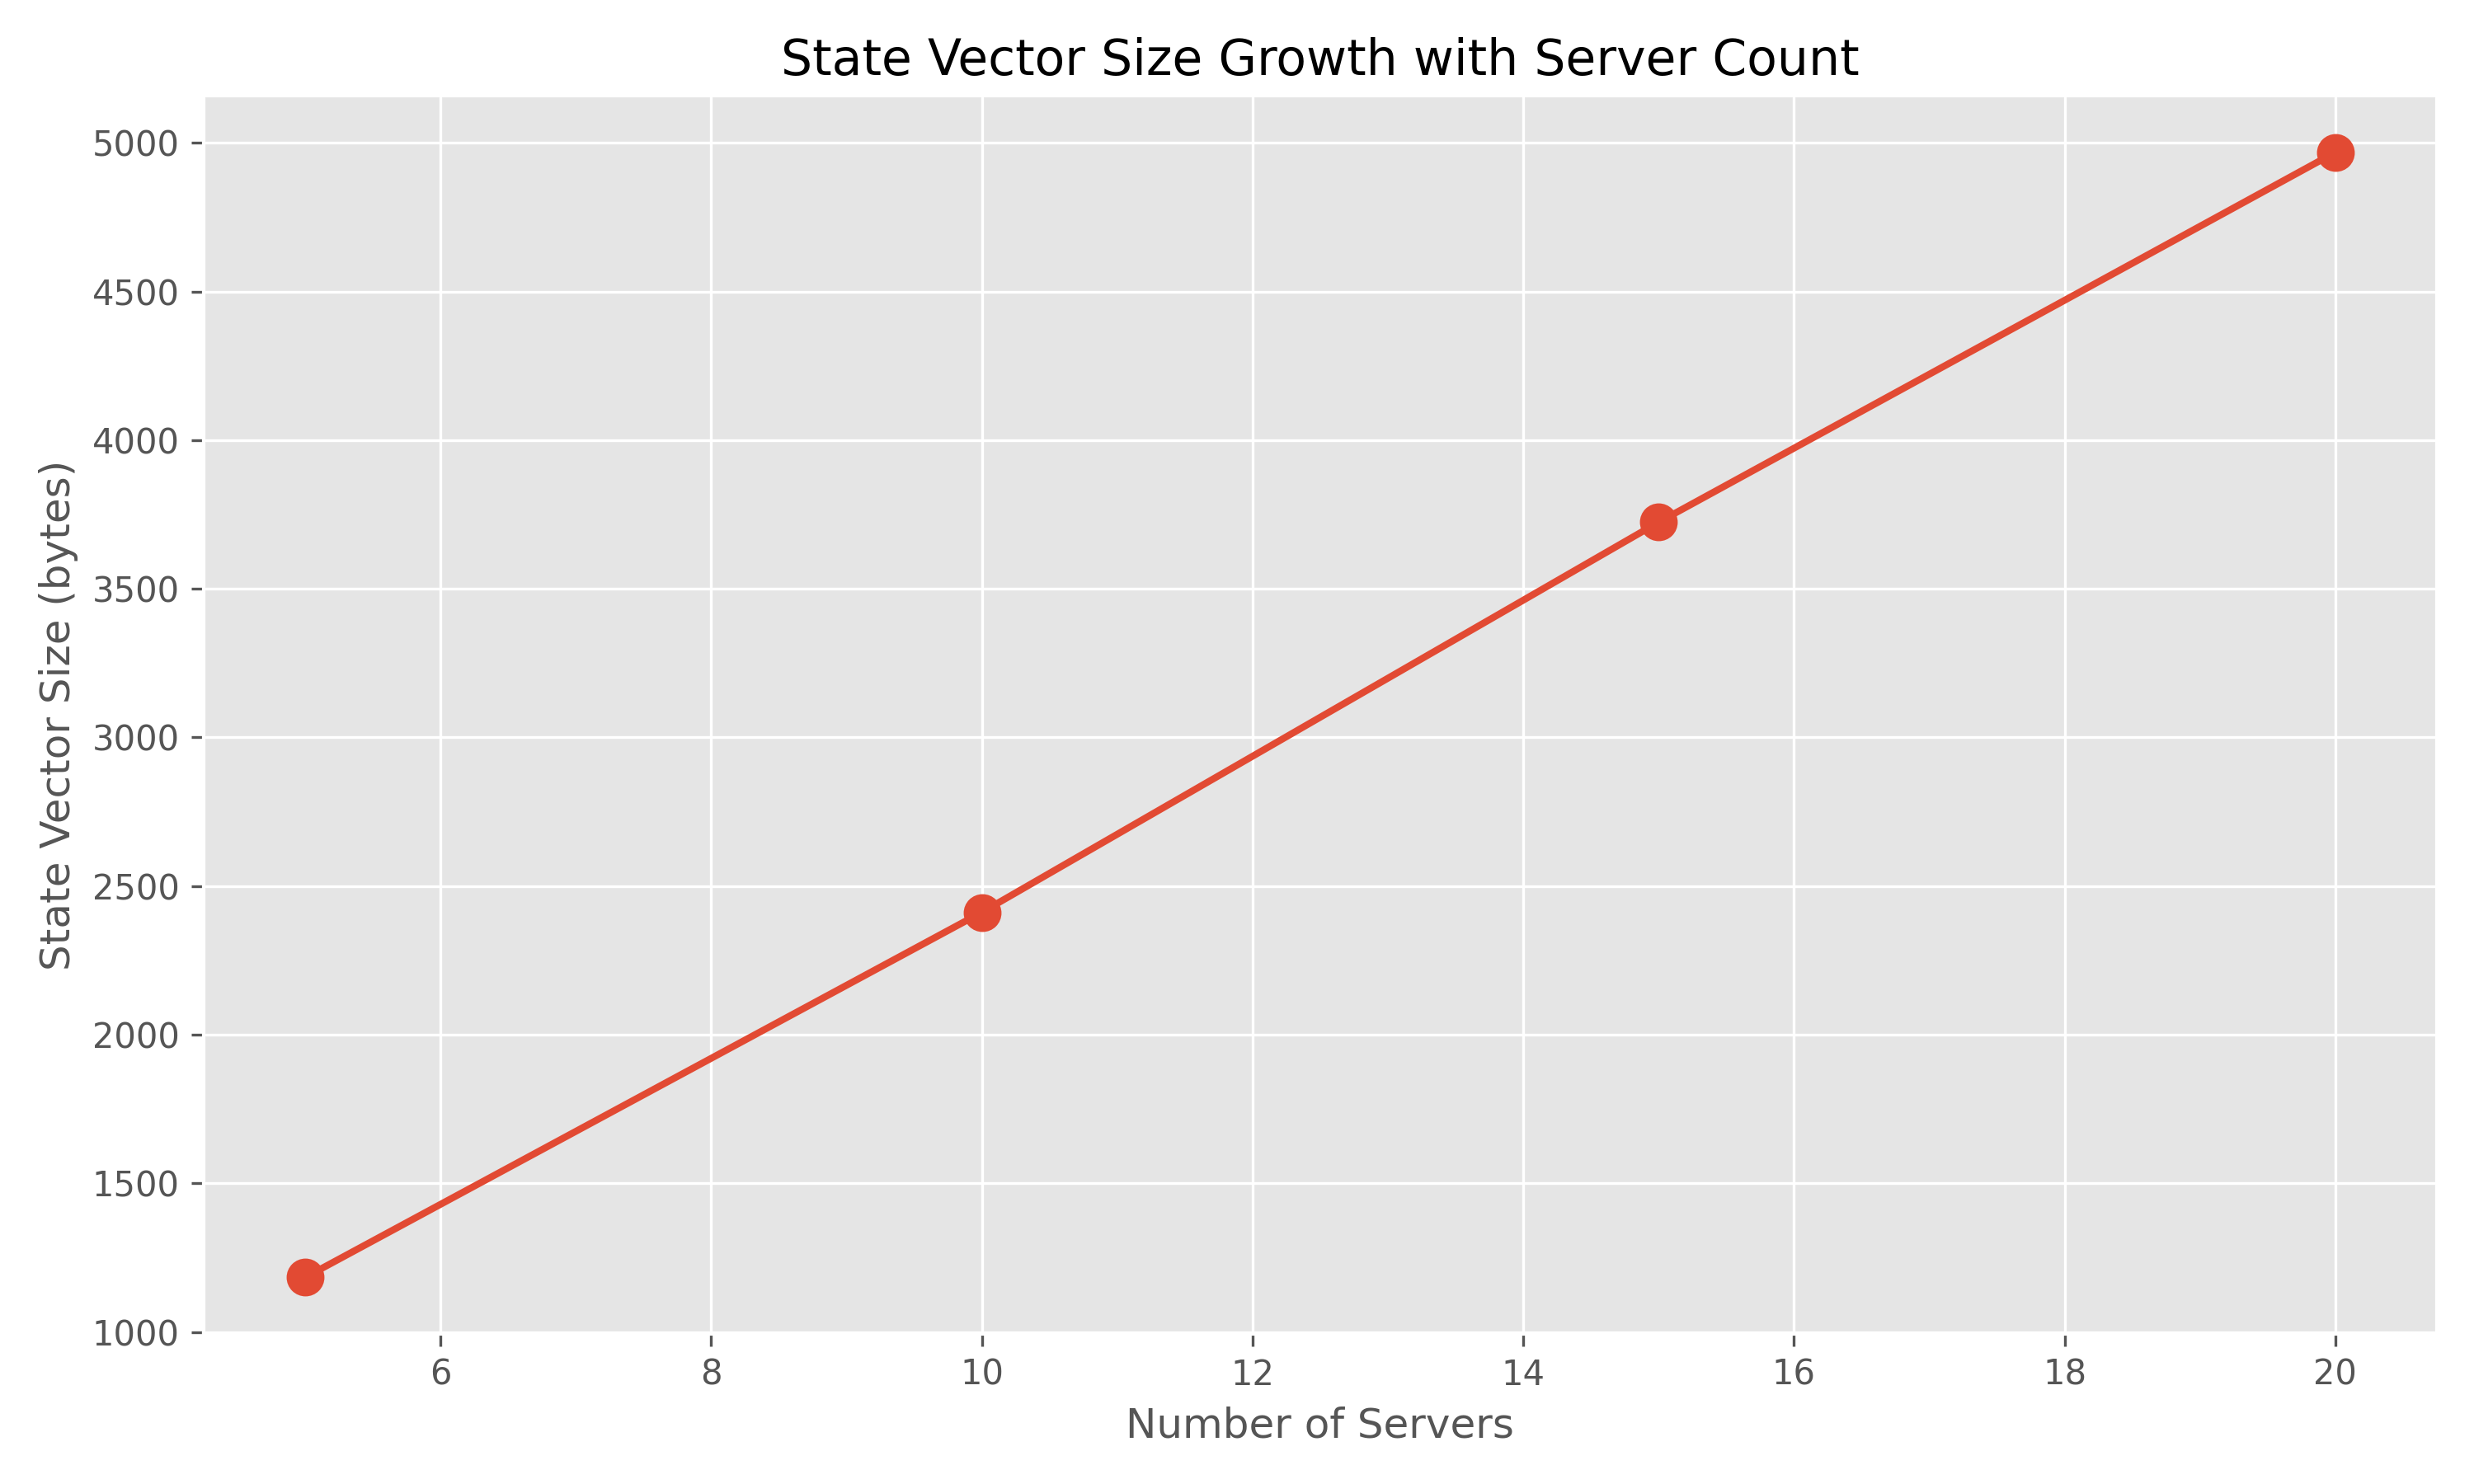
\includegraphics[width=0.8\textwidth]{Images/state_vector_size.png}
    \caption{Linear growth of state vector size with increasing server count. The state vector grows by approximately 252 bytes per additional server.}
    \label{fig:state-vector}
\end{figure}

Figure \ref{fig:state-vector} illustrates the linear growth pattern of state vector size as the number of servers increases from 5 to 20. This predictable growth pattern confirms our observation that each additional server increases the state vector by approximately 252 bytes, enabling accurate prediction of memory requirements for larger configurations.

\begin{figure}[htbp]
    \centering
    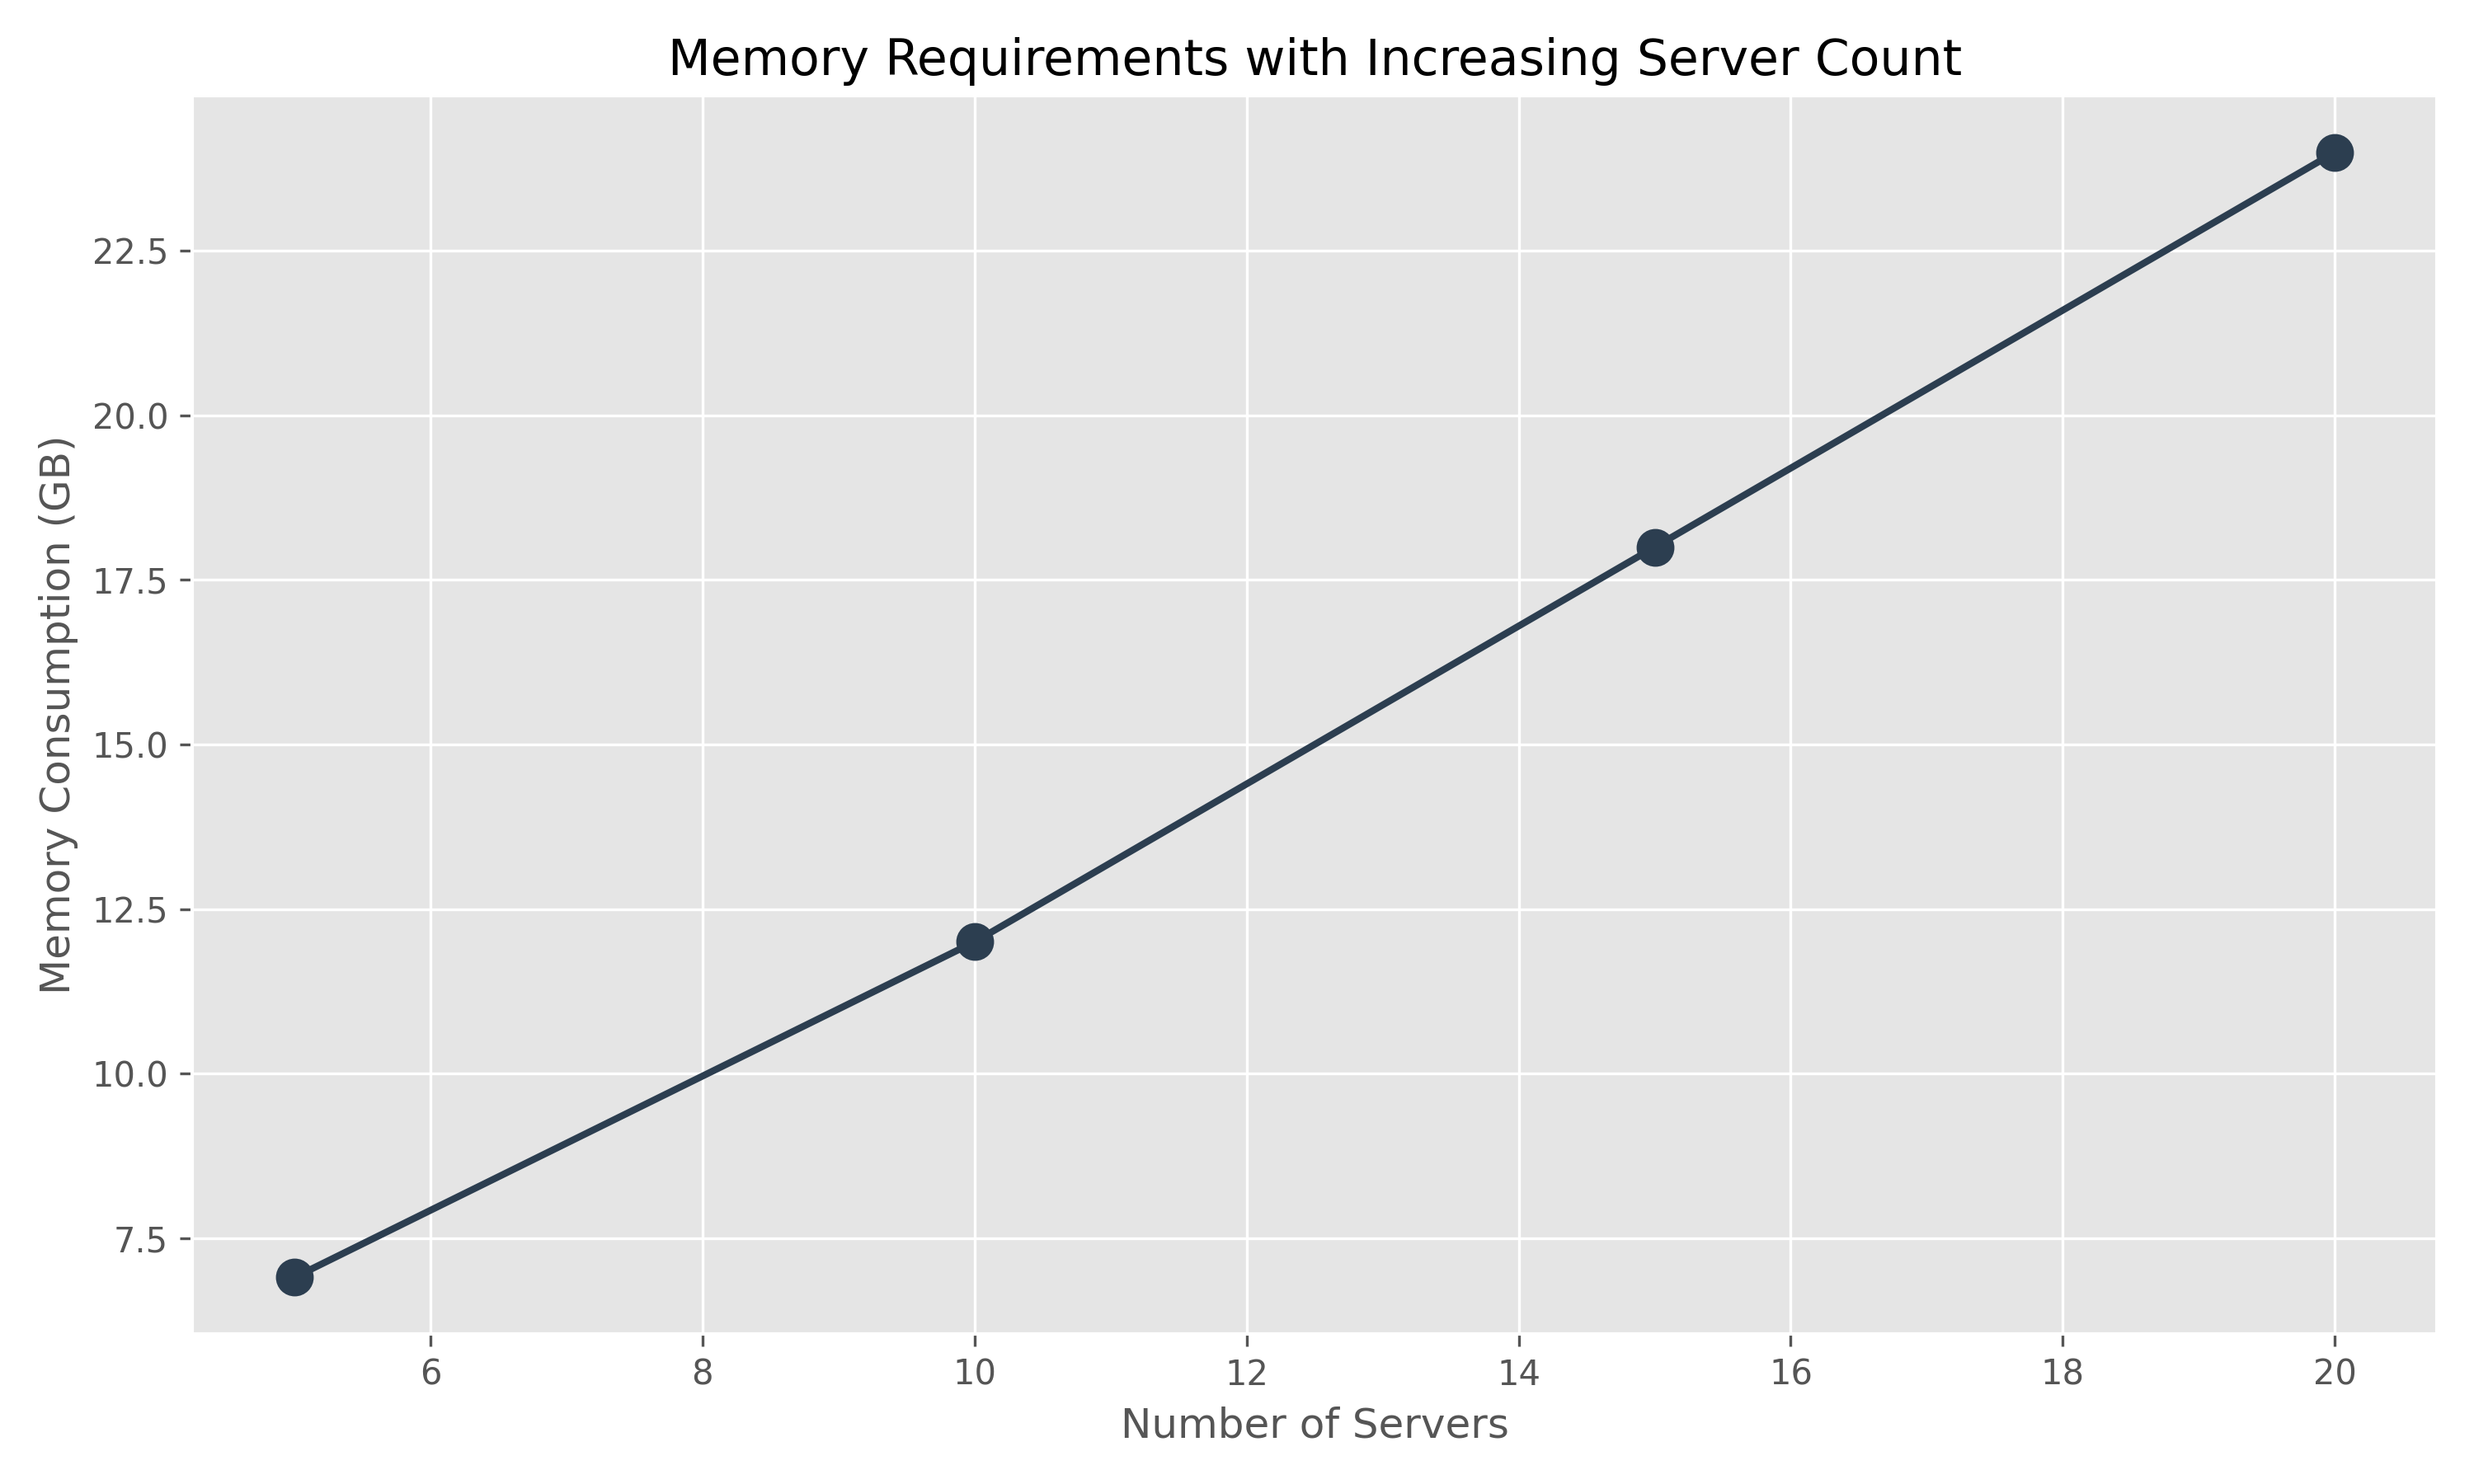
\includegraphics[width=0.8\textwidth]{Images/memory_consumption.png}
    \caption{Memory consumption scaling with server count. The nearly linear relationship indicates predictable resource requirements for verification of larger configurations.}
    \label{fig:memory-consumption}
\end{figure}

The corresponding memory requirements (Figure \ref{fig:memory-consumption}) demonstrate similar scaling behavior, with memory consumption increasing from approximately 7GB with 5 servers to 24GB with 20 servers. The consistent growth pattern supports our conclusion that memory requirements scale predictably with server count.

\begin{figure}[htbp]
    \centering
    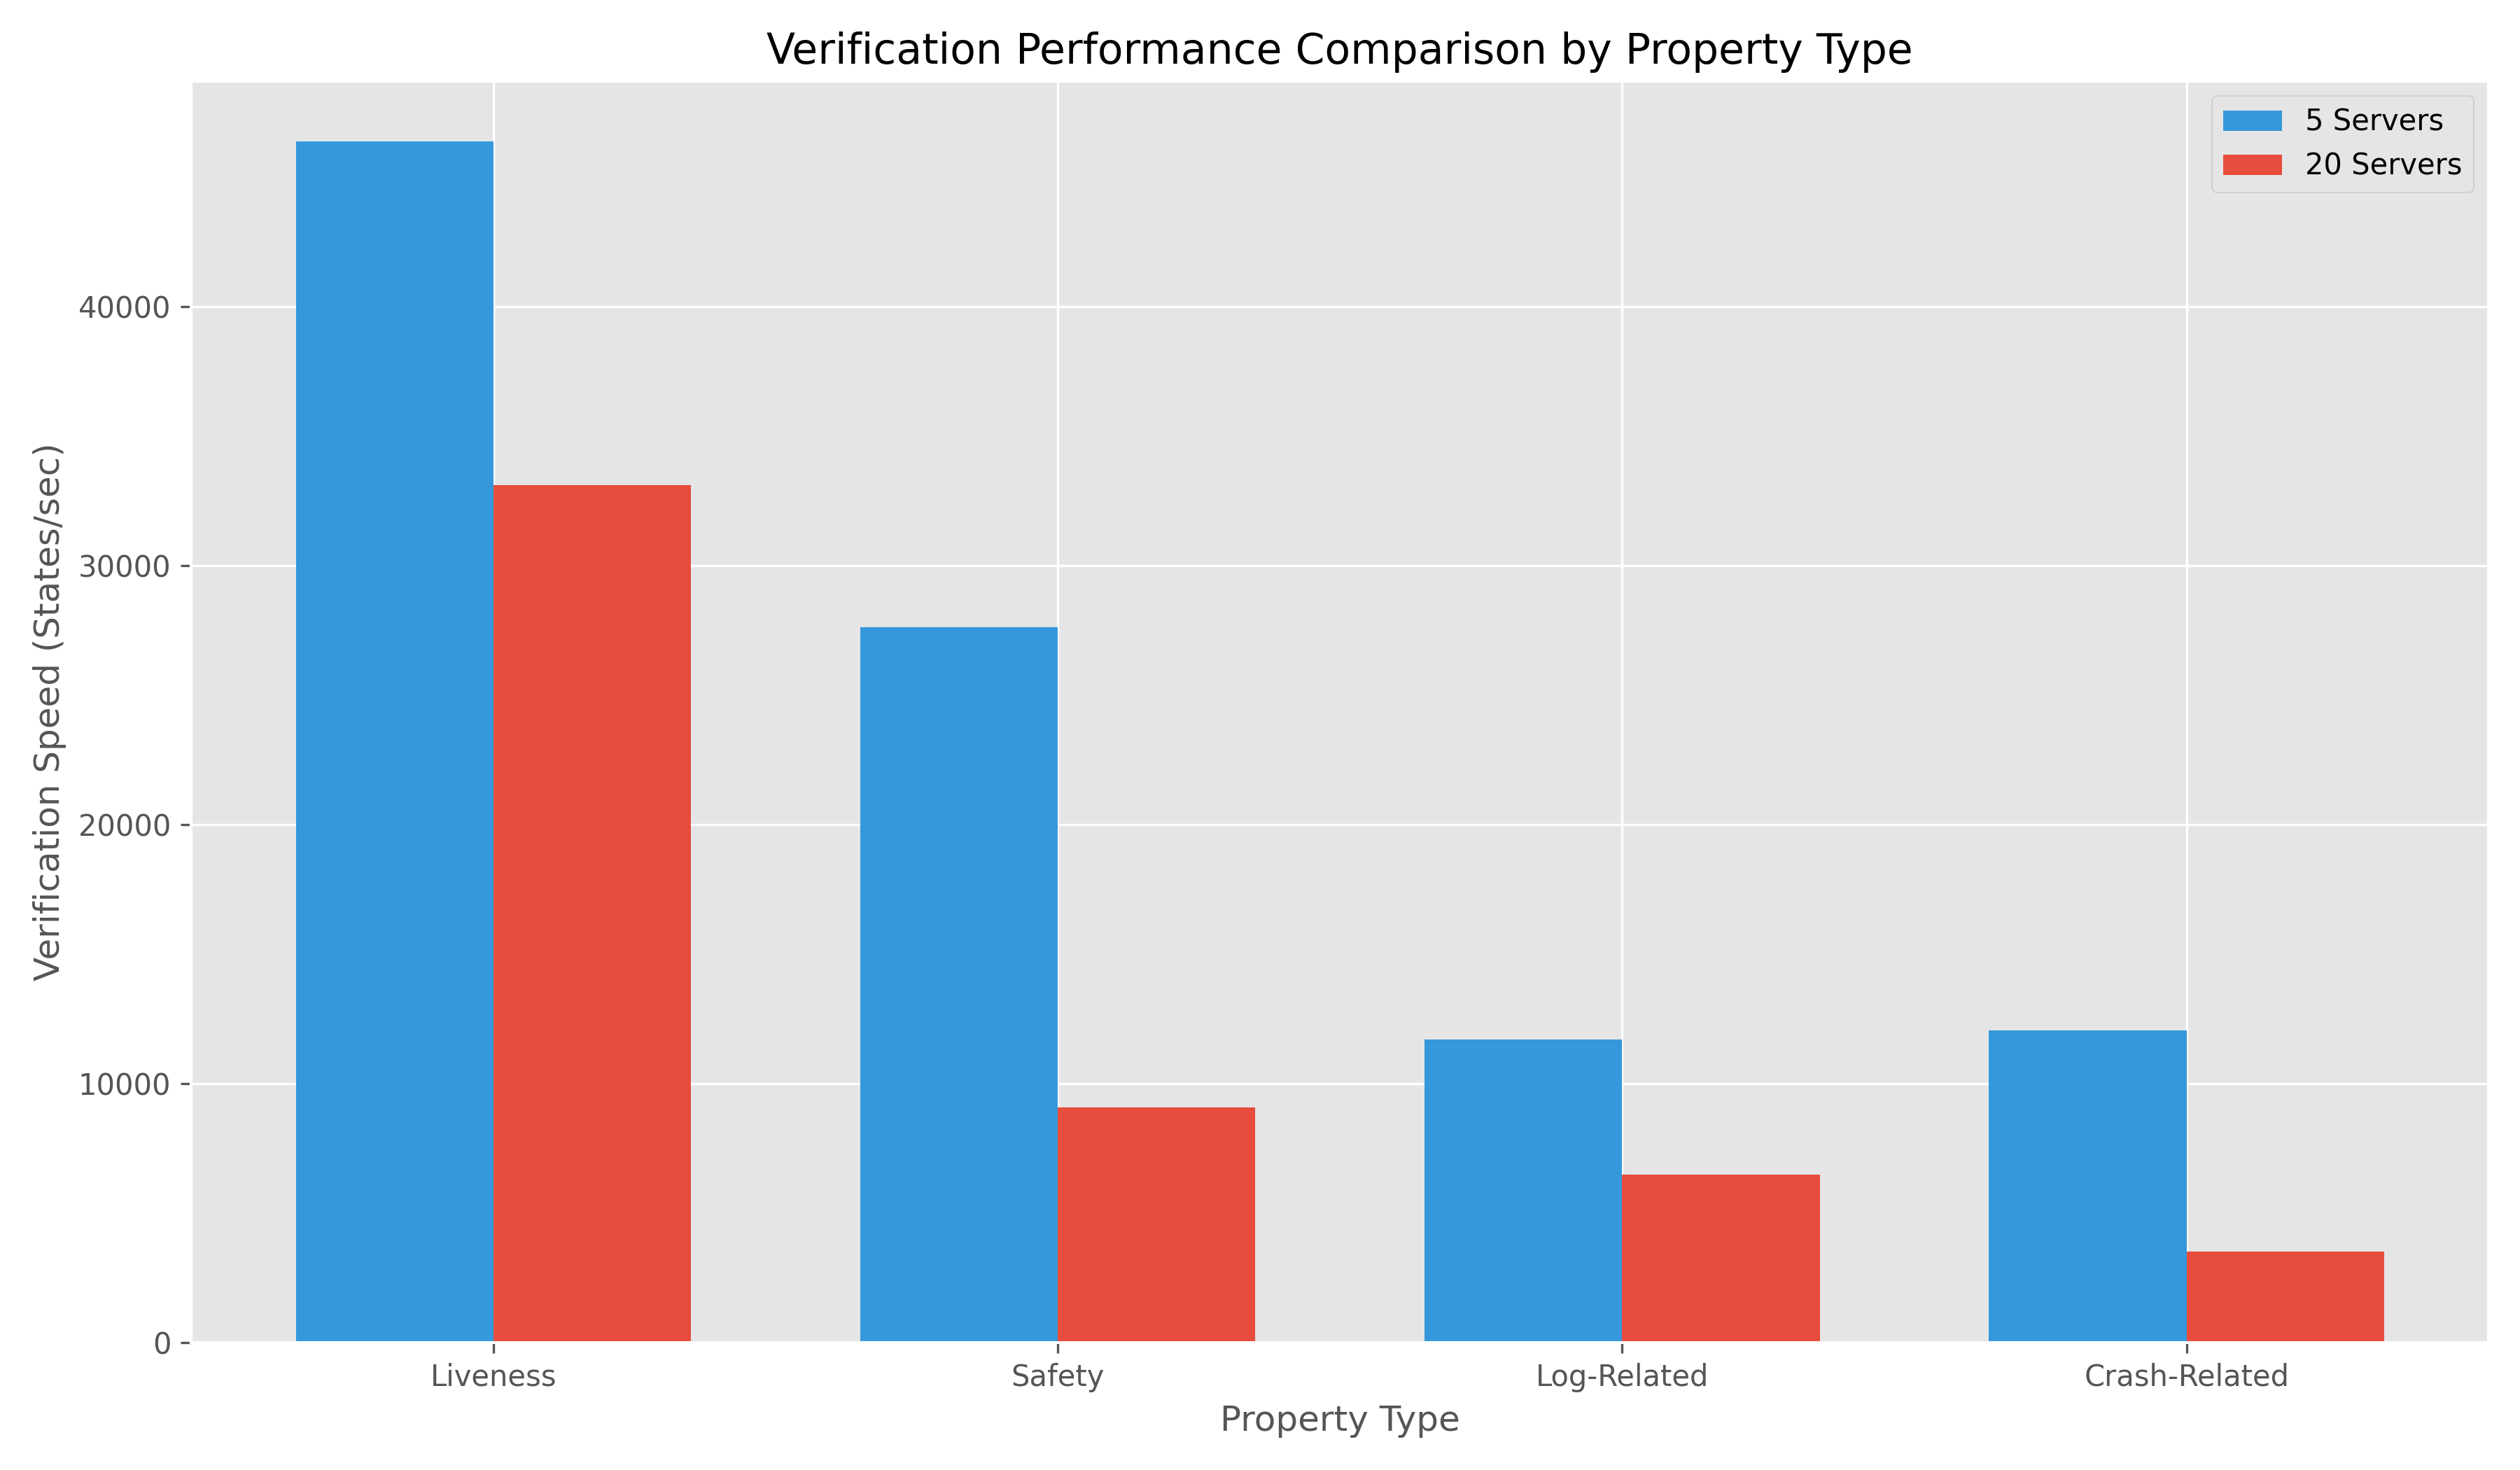
\includegraphics[width=0.9\textwidth]{Images/verification_performance.png}
    \caption{Verification speed comparison between 5-server and 20-server configurations for different property types. Liveness properties maintain the highest verification performance even at larger scale.}
    \label{fig:verification-performance}
\end{figure}

Figure \ref{fig:verification-performance} provides a clear comparison of verification speeds between 5-server and 20-server configurations across the four property categories. This visualization emphasizes the substantial performance gaps, particularly for crash-related properties, which experience the most significant slowdown when scaling to larger configurations.

\begin{figure}[htbp]
    \centering
    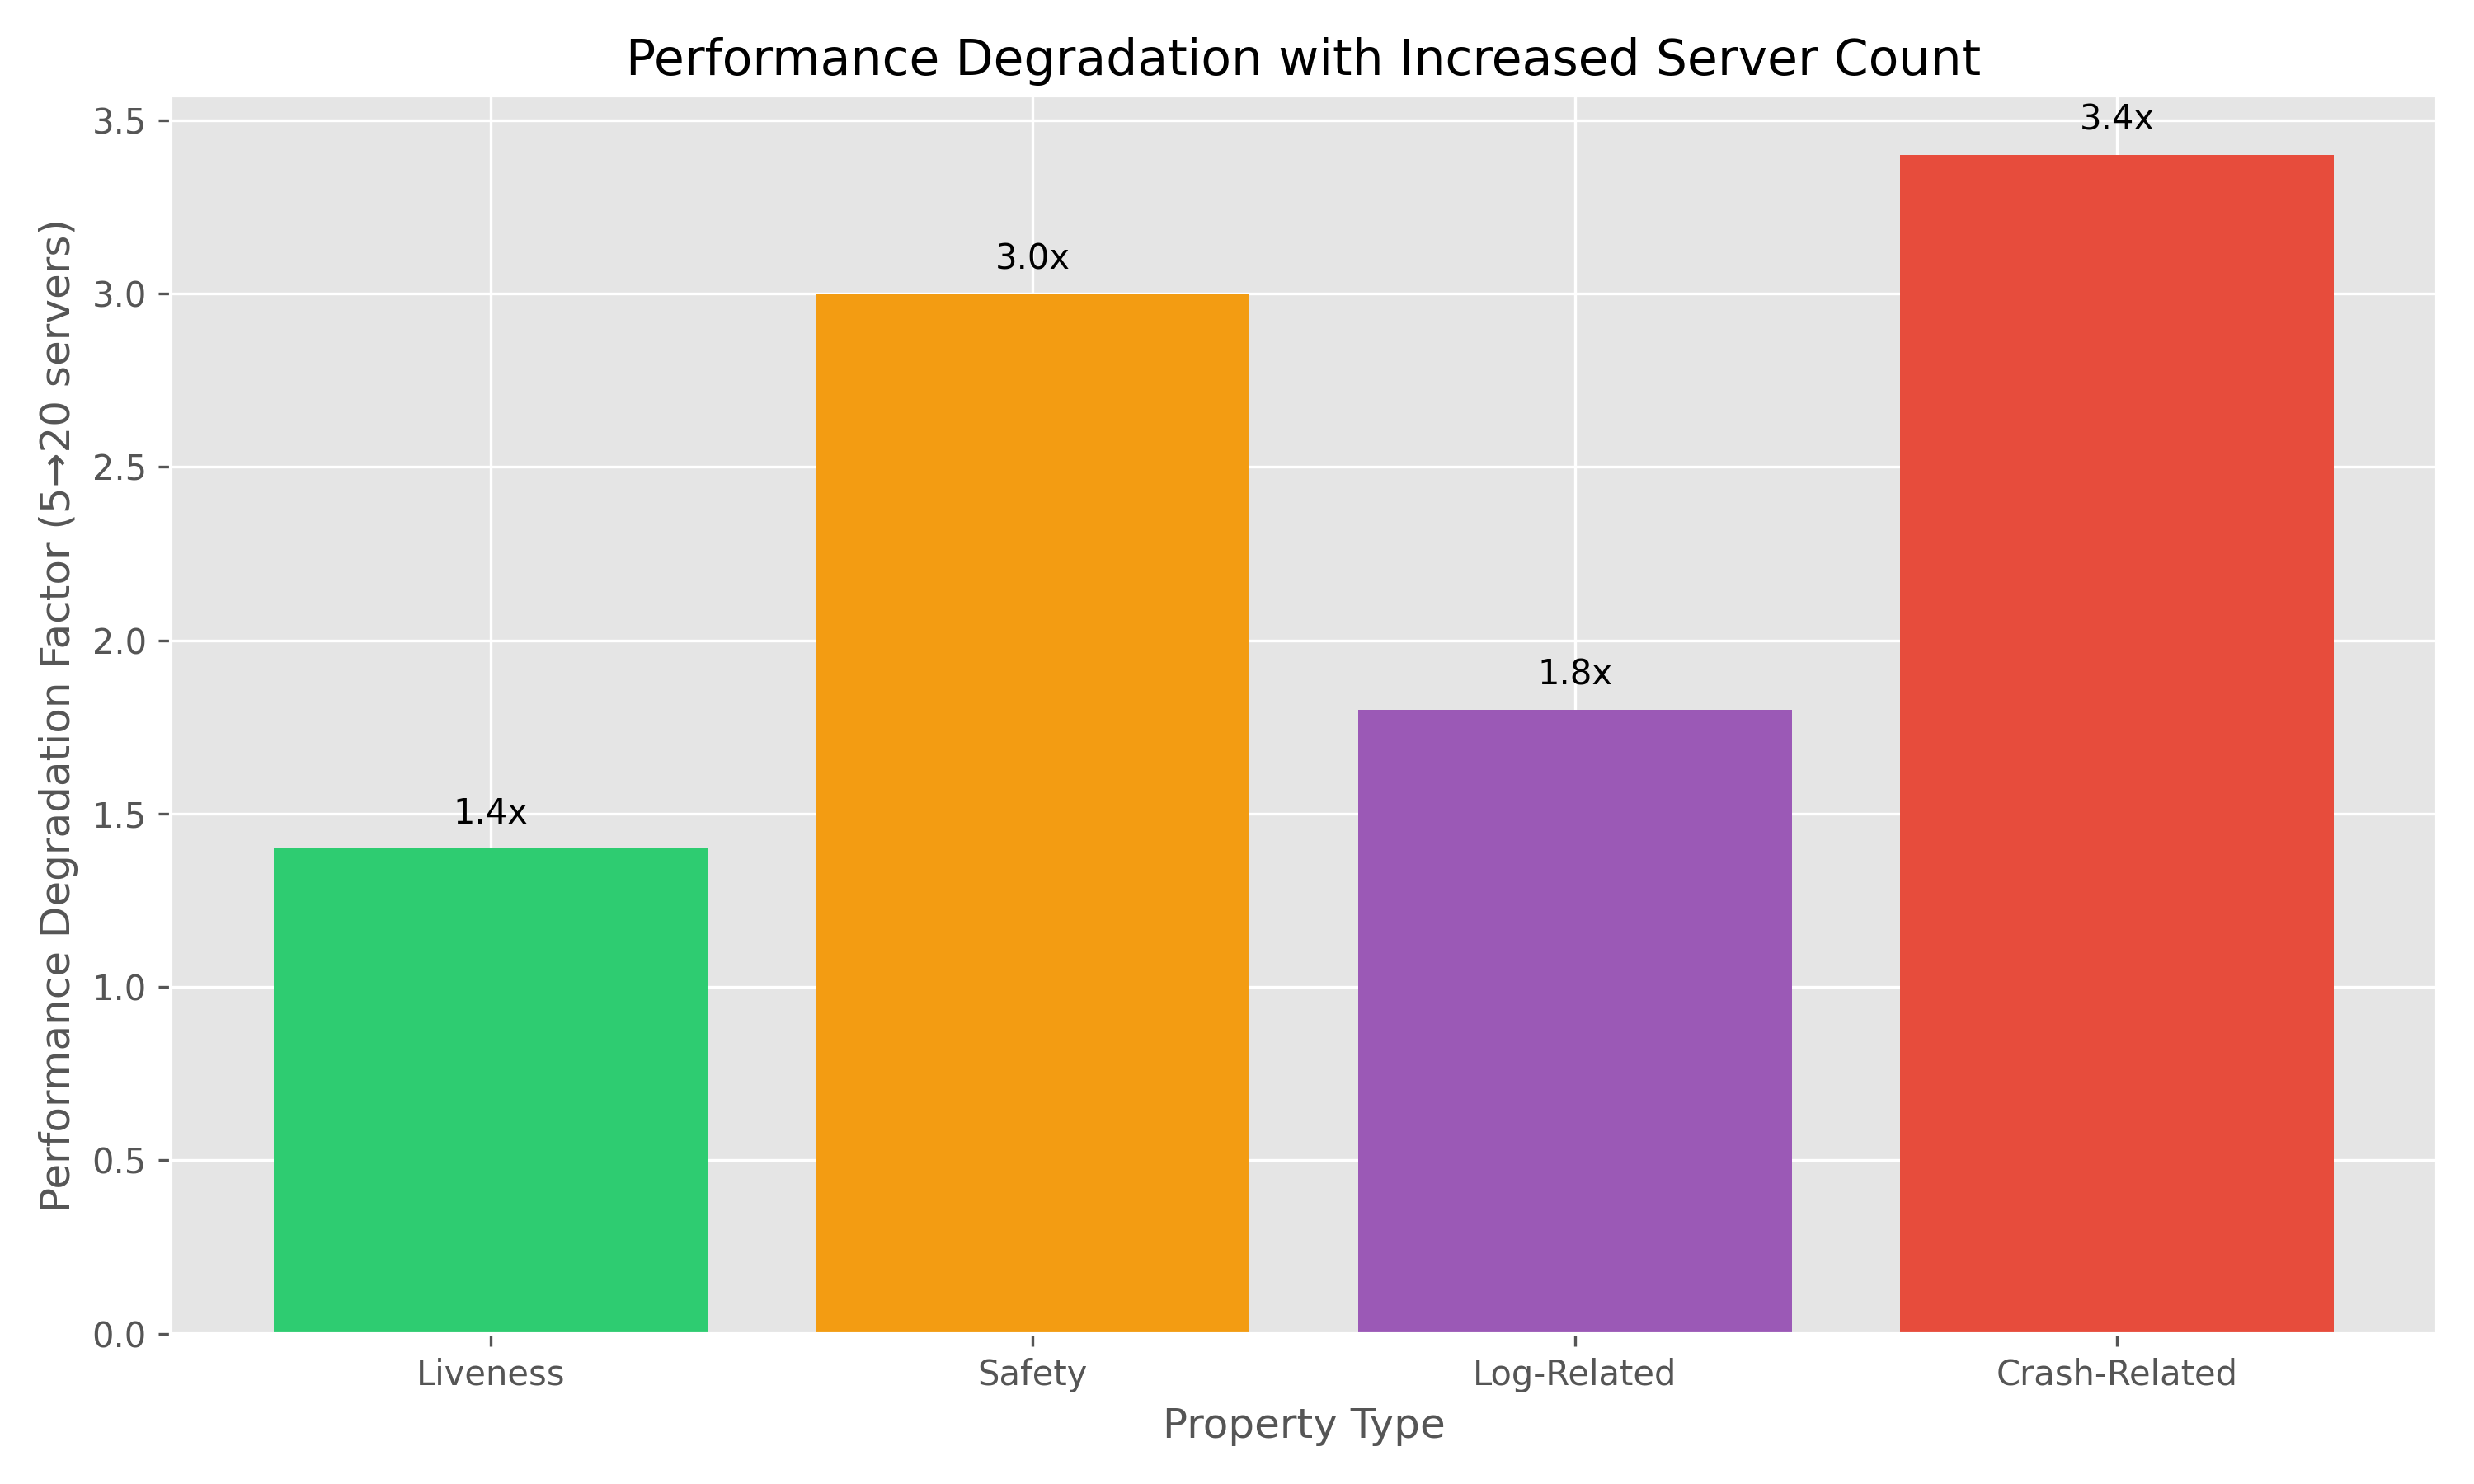
\includegraphics[width=0.8\textwidth]{Images/performance_degradation.png}
    \caption{Performance degradation factors by property type when scaling from 5 to 20 servers. Crash-related properties experience the most significant verification slowdown (3.4x), while liveness properties degrade more gracefully (1.4x).}
    \label{fig:performance-degradation}
\end{figure}

The non-uniform degradation patterns are quantified in Figure \ref{fig:performance-degradation}, which shows that crash-related properties suffer a 3.4x performance degradation when scaling from 5 to 20 servers, compared to only 1.4x for liveness properties. This visualization reinforces our finding that property complexity interacts with system scale in different ways.

\begin{figure}[htbp]
    \centering
    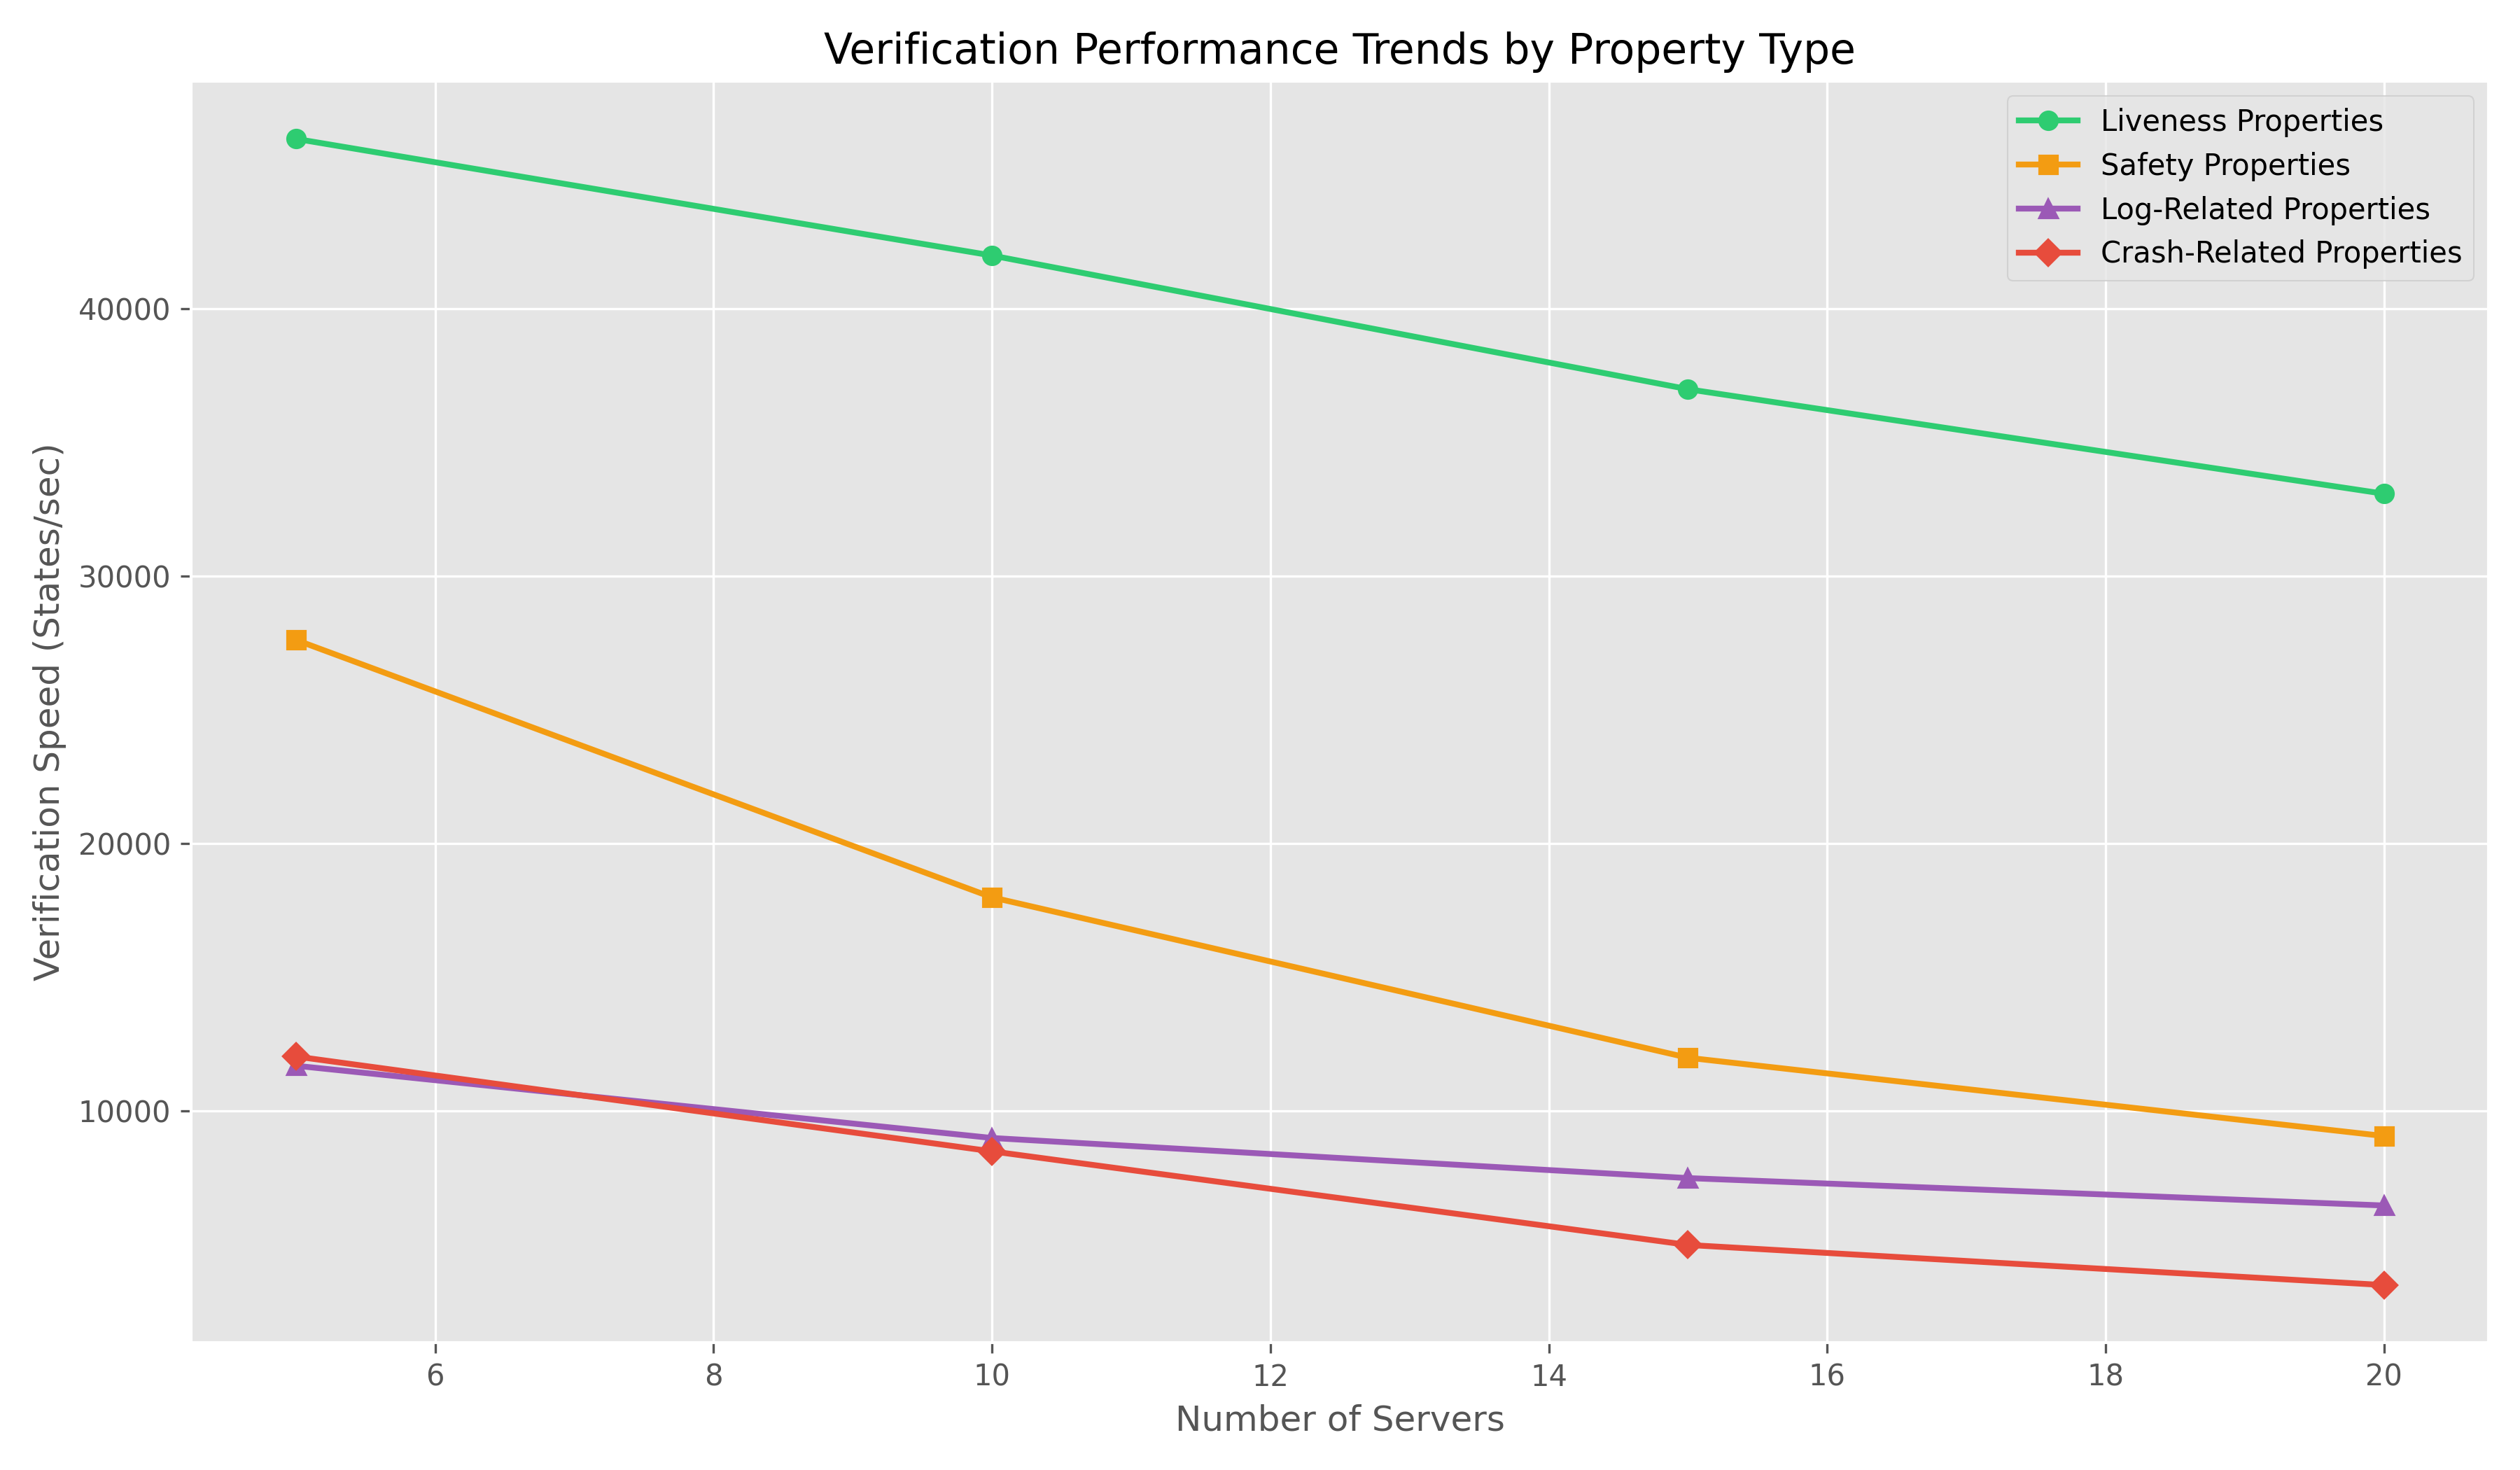
\includegraphics[width=0.95\textwidth]{Images/performance_trends.png}
    \caption{Verification speed trends across server configurations by property type. Liveness properties consistently outperform other property types, while crash-related properties show the steepest performance decline.}
    \label{fig:performance-trends}
\end{figure}

Finally, Figure \ref{fig:performance-trends} provides a comprehensive view of verification performance trends across all server configurations (5, 10, 15, and 20 servers) for each property type. The divergent trends clearly illustrate that verification complexity does not scale uniformly across property types, with the performance gaps widening significantly at larger scales. This insight has important implications for verification strategy, suggesting that different approaches should be used depending on the type of property being verified.

\subsection{Scalability Limitations and Challenges}
\label{sec:scalability}

Our verification efforts encountered several scalability challenges:

\begin{itemize}
    \item \textbf{State Space Explosion}: The number of possible system states grows exponentially with server count.
    
    \item \textbf{Memory Constraints}: Verifications with higher server counts quickly exceeded available memory.
    
    \item \textbf{Search Depth Limitations}: The default search depth (999) proved insufficient for complete verification.
    
    \item \textbf{Time Constraints}: Verification times increased significantly with server count, with runs for n=15 taking over 1,700 seconds for partial verification.
\end{itemize}

To address these limitations, we employed several strategies from the literature \cite{Holzmann97, Garavel}:
\begin{itemize}
    \item State compression, achieving 95-98\% compression efficiency
    \item Partial order reduction to minimize redundant state exploration
    \item Atomic blocks to reduce interleaving where appropriate
\end{itemize}

Despite these optimizations, complete verification remains challenging for larger server configurations.

\subsection{Summary of Findings}
\label{sec:findings}
Our verification results support several key conclusions:
\begin{enumerate}
    \item The Raft consensus algorithm, as modeled in our extended implementation, preserves all safety properties across different server configurations.
    
    \item The memory and computational requirements for comprehensive verification grow significantly with server count, highlighting the challenge of formal verification for realistic distributed systems.
    
    \item For low search depth (100), we achieved complete verification with no safety violations detected, and the verification process terminated normally without errors, providing strong evidence for the correctness of our implementation.
    
    \item For high search depth (1000), no safety violations were detected throughout partial verification until memory was exhausted, further supporting correctness across a larger but incomplete state space.
    
    \item Even partial verification provides valuable assurance by checking millions of states without finding counterexamples.
    
    \item Our model's handling of crashed nodes maintains safety properties, supporting Raft's claim of crash fault tolerance.
    
    \item The implementation of heartbeat message logic proved effective in maintaining leader authority and preventing unnecessary elections, a key aspect of Raft's stability guarantees.
    
    \item Our verification of heartbeat-specific properties demonstrates that: (a) the heartbeat effectiveness property prevents candidates from prematurely transitioning to follower state without proper validation, and (b) the heartbeat stability property ensures leaders with a quorum maintain their position consistently, showing high verification rates even with increasing server counts.

    \item Different property types exhibit varying verification performance characteristics, with liveness properties being more efficiently checked than crash-related properties as detailed in Section \ref{sec:trends}.
\end{enumerate}

These results demonstrate that our extended Raft model with configurable server count, crash handling, and dedicated network layer correctly implements the protocol's safety guarantees, even as the verification process becomes increasingly resource-intensive with larger configurations.

    
    \chapter{Conclusion}
    \label{sec:conclusion}

    In this work, we have presented a comprehensive formal verification approach for the Raft consensus algorithm using the SPIN model checker and Promela modeling language. Our analysis focused on rigorously testing and checking the safety guarantees of Raft across a range of server configurations, from 5 servers up to larger clusters with 20 servers, with both complete and partial verification strategies.
    
    The verification yielded two key results that support Raft's correctness:
    \begin{itemize}
        \item With low search depth (100), we achieved \textbf{complete verification} that terminated normally with no errors or safety violations found, validating the algorithm's correctness within the explored state space.
        \item With high search depth (1000), we achieved \textbf{extensive partial verification} where no violations were found until memory was exhausted, supporting correctness across a significantly larger but incomplete state space.
    \end{itemize}
    
    These results provide strong evidence for the correctness of the Raft algorithm because no safety violations were found among millions of states investigated across both verification approaches. We were able to check significant properties like Election Safety, Log Matching, State Machine Safety, and various crash recovery conditions as described in Section \ref{sec:safety_properties}. These results support that Raft's design achieves its goal of guaranteeing consistency in the presence of node failures, providing assurance of the reliability of the algorithm for distributed systems applications.

Our findings underscore the inherent difficulty of complete exhaustive verification of distributed consensus protocols. The state space increases exponentially with the number of servers, resulting in astronomical memory requirements and verification time explosion as shown in our analysis in Section \ref{sec:verification_performance}. Even when optimizations such as state compression and partial order reduction are used, complete exhaustive verification is computationally impractical for large configurations. However, our successful partial verification across diverse system configurations and substantial state space exploration provides a high degree of confidence in the algorithm's correctness.
    
    This research makes several key contributions:
    
    \begin{itemize}
        \item An extended Promela model of Raft that supports arbitrary server counts, improving on previous work \cite{Qx1} that was limited to fixed configurations.
        
        \item Formal verification of Raft's safety properties with different cluster sizes, demonstrating the algorithm's correctness scales with the number of nodes.
        
        \item Detailed performance analysis that quantifies the verification challenges as system complexity increases.
        
        \item Confirmation that our implementation of crash handling preserves the algorithm's safety guarantees, validating Raft's crash fault tolerance.
        
        \item Novel insights into property-specific verification performance, revealing that liveness properties scale more efficiently (1.4x degradation) than crash-related properties (3.4x degradation) as server count increases.
    \end{itemize}
    
    For future work, we identify several promising directions. First, exploring advanced state space reduction techniques could enable more complete verification of larger configurations. Second, extending the model to incorporate Byzantine fault tolerance \cite{Qx6, Qx8, Castro} would expand its applicability to blockchain and other security-critical systems. Finally, developing property-specific optimization approaches based on our degradation analysis in Section \ref{sec:trends} could significantly improve verification efficiency for complex distributed systems.
    
    Overall, our findings reinforce the potential of formal methods as a powerful approach for analyzing and improving distributed systems, while also highlighting the continuing need for innovation in verification techniques to address the scalability challenges inherent in these complex systems. The observed patterns in verification performance across different property types suggest that tailored verification strategies for different classes of properties could lead to more efficient formal verification of large-scale distributed systems in the future.
    